\chapter{Review of Related Literature}
\label{sec:rrl} 

\section{ddPCR Quantification tools}
\label{sec:dpcrclassifiers}

Because of the partitioning nature of droplet dPCR, it is more sensitive in detecting target nucleic acid. Detection is crucial in analyzing low-copy molecules such as in viruses like the HIV-1 DNA and 2-LTR circles \cite{Henricha2012}. As mentioned in section \ref{sec:backgroundstudy}, the dPCR workflow may introduce several sources of variation, including human error in pipetting techniques, to the use of diluting DNA samples to lessen the Poisson variability in a positive partition. This section explores the statistical methods in current quantification systems of single-channel dPCR experiments. The terms ddPCR (droplet dPCR) and dPCR are synonymous and may be used interchangeably.

\subsection{Bio-Rad Quantasoft}
\label{sec:ddpcrsystem}
% TODO : Mention the other ddPCR systems mentioned in Dong paper (Raindrop and QuantStudio) %
The most common method in classifying positive and negative droplets is by enforcing a hard threshold. Generally, all droplets with a fluorescence amplitude greater than this threshold are then classified as positive, and negative otherwise. 

One popular tool incorporated with automatic thresholding is the QuantaSoft software. The QuantaSoft software is the dPCR analysis tool that comes with the Bio-Rad droplet dPCR System package. It allows for the setting up of sample and experiments, running and controlling the instrument, and finally, the analysis of the nucleic acid concentration \cite{Bio-Rad2019}. According to the Bio-Rad Laboratories website (https://www.bio-rad.com), it has been a leading product developer for 65 years in the research fields of life science and clinical diagnostics. Among its popular focus areas, dPCR is one of its most featured technology, providing ddPCR instruments; kits, reagents and assays; and other consumables. Several studies in hospitals \cite{Lopez2016,Chen2018,Abed2017,Tagliapietra2020}, public health \cite{Hussain2017,Nystrand2018}, food safety \cite{Chen2020,Capobianco2020,Basanisi2020}, up to environmental quality \cite{Hamaguchi2018,Jahne2020,Dobnik2016,Mauvisseau2019} have found the Bio-Rad QuantaSoft dPCR systems useful for their analyses. 

Of all the QuantaSoft software features, the focus of this section is on its threshold setting. By default, QuantaSoft sets an automatic threshold to the single-well or multiple-well amplitude data; a demonstration is shown in \figref{fig:demoQuantThreshold}. As with other automated tools, its documentation recommends reviewing this threshold to make changes if needed; and thus, manually setting the threshold is also allowed. Unfortunately, the calculation of the automatic threshold is not publicly available.

\begin{figure}[h]
    \centering
    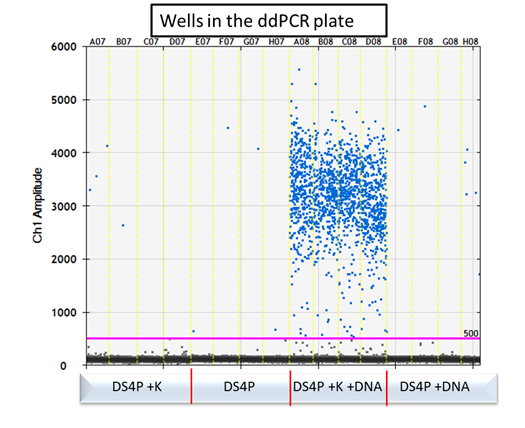
\includegraphics[max size={\textwidth}{\textheight}]{quantasoftThreshold.png}
    \caption[QuantaSoft threshold from a study]{QuantaSoft threshold in pink line from \cite{hussainThreshold}}
        \label{fig:demoQuantThreshold}
\end{figure}

The evaluation of the QuantaSoft software show satisfactory results from the food safety study of \citeA{Basanisi2020}, whereby nine pure meat samples were discriminated with 100\% diagnostic accuracy, sensitivity, and specificity. However, upon checking the authenticity of twenty commercially available meat products, twelve samples were said to contain DNA traces of other animals not declared. Among the several reasons for this high detection, \citeA{Basanisi2020} emphasizes the need for a highly sensitive and specific test at the molecular level.

Assessing the QuantaSoft software's ability to classify droplets, it was shown that for samples exhibiting a substantial amount of intermediate fluorescence, the system fails to determine a threshold (outputs "No call"). This was the case in the bacteria study of \shortciteA{Dreo2014}, that were ran on very high concentrations. In the case of low bacteria concentrations, droplets near the negative droplets were classified as positives. Similarly, \shortciteA{Witte2016} has observed around 10\% positive count differences between low and high threshold settings using the same data. The heavy presence of rain in their assay prevented a clear threshold value.  Both these studies noted that the QuantaSoft software requires a well-optimized assay with good discrimination of positive and negative droplets for its threshold to be reliable. 


\subsection{Manual Global Threshold (MTg)}
\label{sec:manthreshold}
As opposed to the automatic threshold, \citeA{Dreo2014} proposes setting a manual global threshold (MTg) determined by no template control (NTC) samples. This takes into consideration that individual assays behave differently, and could require expert intervention. As a standard approach, the threshold for a well-optimised assay was defined as the NTC mean + 6 standard deviations; on the other hand, a noisy assay had its threshold set above the highest value in NTC samples. It is expected in the latter case that the sensitivity would be lower, due to its high threshold. However, the paper claims that this resulted in high analytical sensitivity for that assay. A major disadvantage in this approach is the lack of a clear definition or guideline in setting the MTg; this consequently will cause reproducibility issues for succeeding experiments and external researchers.


\subsection{definetherain}
\label{sec:knn}
Based on the research papers curated by \citeA{Peterson:2009}, K-nearest-neighbor (KNN) is a unsupervised clustering approach that should be among the first methods considered for data with little to no information about its distribution. This clustering method operates on the chosen distance measure — commonly the Euclidean distance — between the observations. Due to its simplicity, data from various fields have applied KNN such as in a movie recommendation system \cite{Ahuja2019}, climate classification \cite{Shi2020}, breast cancer diagnostics \cite{Mittal2019}, among others.

The positive and negative droplet classification can be framed as a clustering problem. An open-source tool developed by \shortciteA{Jones2014}, called definetherain, utilizes the KNN algorithm in identifying rain droplets. According to their research, they claim that definetherain is accurate in estimating assays with low template numbers, which is particularly applicable in research fields such as the HIV-1 cure research. definetherain follows these steps for classification:
\begin{enumerate}
    \item Setup a positive control sample of known input copy numbers. 
    \item Cluster the droplets using kNN with \(k=2\). The cluster on the left is the negative cluster, and on the right is the positive cluster. 
    \item Observations between the range of the negative cluster's mean + 3 standard deviations and the positive cluster's mean - 3 standard deviations are classified as rain.
    \item Rain droplets are not included in the final calculation of the concentration estimate.
\end{enumerate}

\begin{figure}[h]
    \centering
    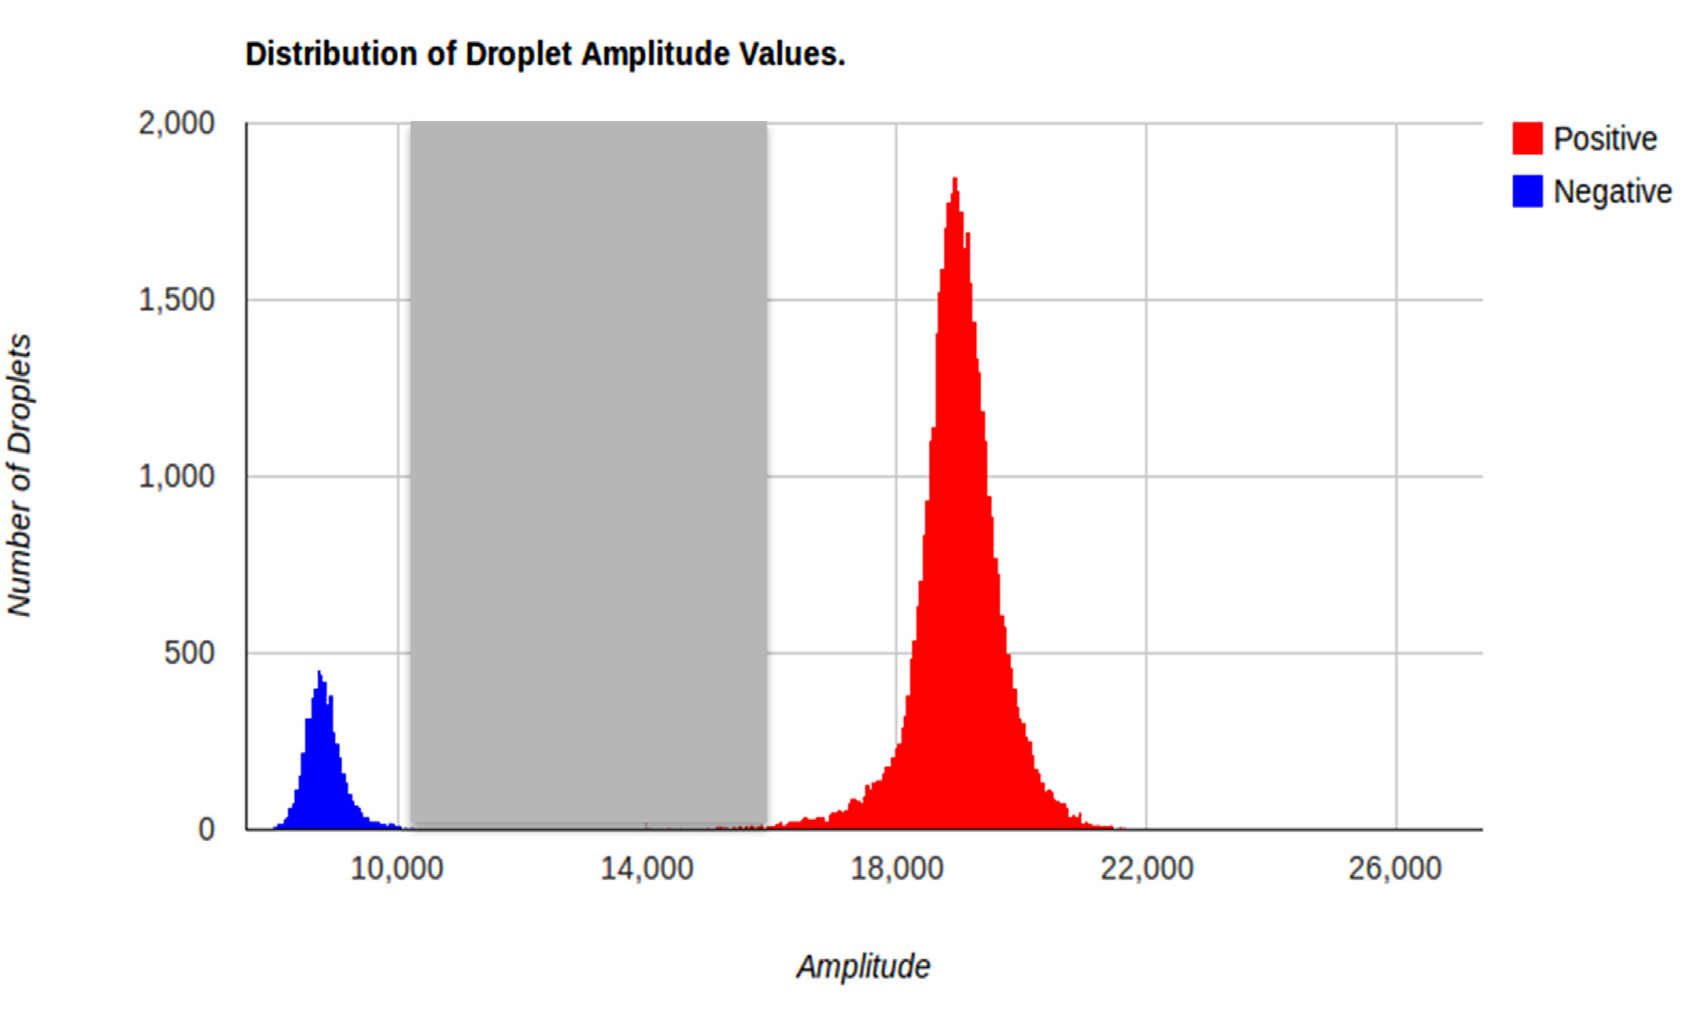
\includegraphics[max size={\textwidth}{\textheight}]{dtrsample.png}
    \caption[Determined thresholds calculated by definetherain]{Determined thresholds calculated by definetherain, reprinted from \cite{jonesThreshold}}
        \label{fig:dtrsample}
\end{figure}

Unlike the other methods discussed here, this tool produces two cutoff values — one for each cluster. The droplets falling between these two values are classified as rain. These cutoff values are solely dependent on the control sample. The disadvantages of the use of a constant threshold for the succeeding target samples is that 1) the control has to be representative of the target, otherwise, concentration estimates would be biased; and 2) the baseline shift of the fluorescence populations are not taken into consideration.

\subsection{Cloudy}
\label{sec:peakdetectionkde}
The research work of \citeA{Lievens2016} has been well cited for its definition of the performance criteria for dPCR assays as well as optimization parameters. The quantification method used in their experiments was available as a supplementary file named "S3\_file.R", which is captioned as their main function to categorize droplets and quantify the concentration. Inside this R code is a function named cloudy. Although "cloudy" was not mentioned in their paper, their algorithm will be refered here as cloudy. 

The cloudy algorithm first determines the fluorescence populations using density peaks, then iteratively estimates the parameters of each population. The droplet categorization depends on its standard deviation distance from a population's mean estimate. The following list summarizes the cloudy algorithm:
\begin{enumerate}
    \item The Guassian kernel density of the fluorescence is estimated with a minimum bandwith of 50
    \item Density peaks are identified using a sliding window approach. The subsequent steps will differ according to if one, two, or more than three peaks were found.  But generally, the proceeding steps are followed.
    \item For each population found through the peaks, its location and spread is initially estimated using the median \(\hat{\mu}\) and \(\hat{\sigma}\). Assuming normality, the latter is estimated as half the peak width at 60-65\% of its maximum height.
    \item Refine the estimates using a reiterative method, first initialized with \(a=4\).
    \item Re-estimate \(\hat{\mu}\) and \(\hat{\sigma}\) using only the observations within \(\hat{\mu} \pm (a \cdot \hat{\sigma})\).
    \item Recalculate \(a=4.55 + 0.35 \cdot \log{k} + 0.045 \cdot \log{k}^2\); where \(k\) is the kurtosis of the distribution
    \item Repeat steps 5-6 until stabilization.
    \item After stabilizing the estimates for all the population, the last step is different when either including or excluding rain in the final categorization. 
    \begin{enumerate}
        \item If rain is included as a category, observations within \(\hat{\mu} \pm (a \cdot \hat{\sigma})\) are then classified as members of that population; observations not falling within any population are classified as rain.
        \item If rain categorization is not of interest, then a threshold \(\theta=\hat{\mu_n} + 1.5 \cdot a_n + \hat{\sigma_n}\) is calculated; where \(n\) is a population.  
    \end{enumerate}

\end{enumerate}

In summary, the cloudy algorithm uses the Gaussian kernel density to detect peaks, which are then considered as populations. Population parameters are then estimated iteratively until convergence. It is worth noting that in its iterative step for estimating the population parameter (step 6), the formula for re-calculating \(a\) is based on the analysis of their in-house data, and should be used with caution when implementing for other unobserved nucleic acid targets. After determining the final population parameters, a range or a single threshold is then calculated for classifying droplets as positive, negative, or optionally, rain. However, the rain classification rule in step 8(a) poses a problem for fluorescence densities that are heavily skewed. \figref{fig:skeweddist} left panel reveals the distribution of negative droplets to be heavily skewed to the right, thereby causing their exclusion to be labeled as negative due to the symmetry of the categorization rule (right panel).

\begin{figure}[h]
    \centering
    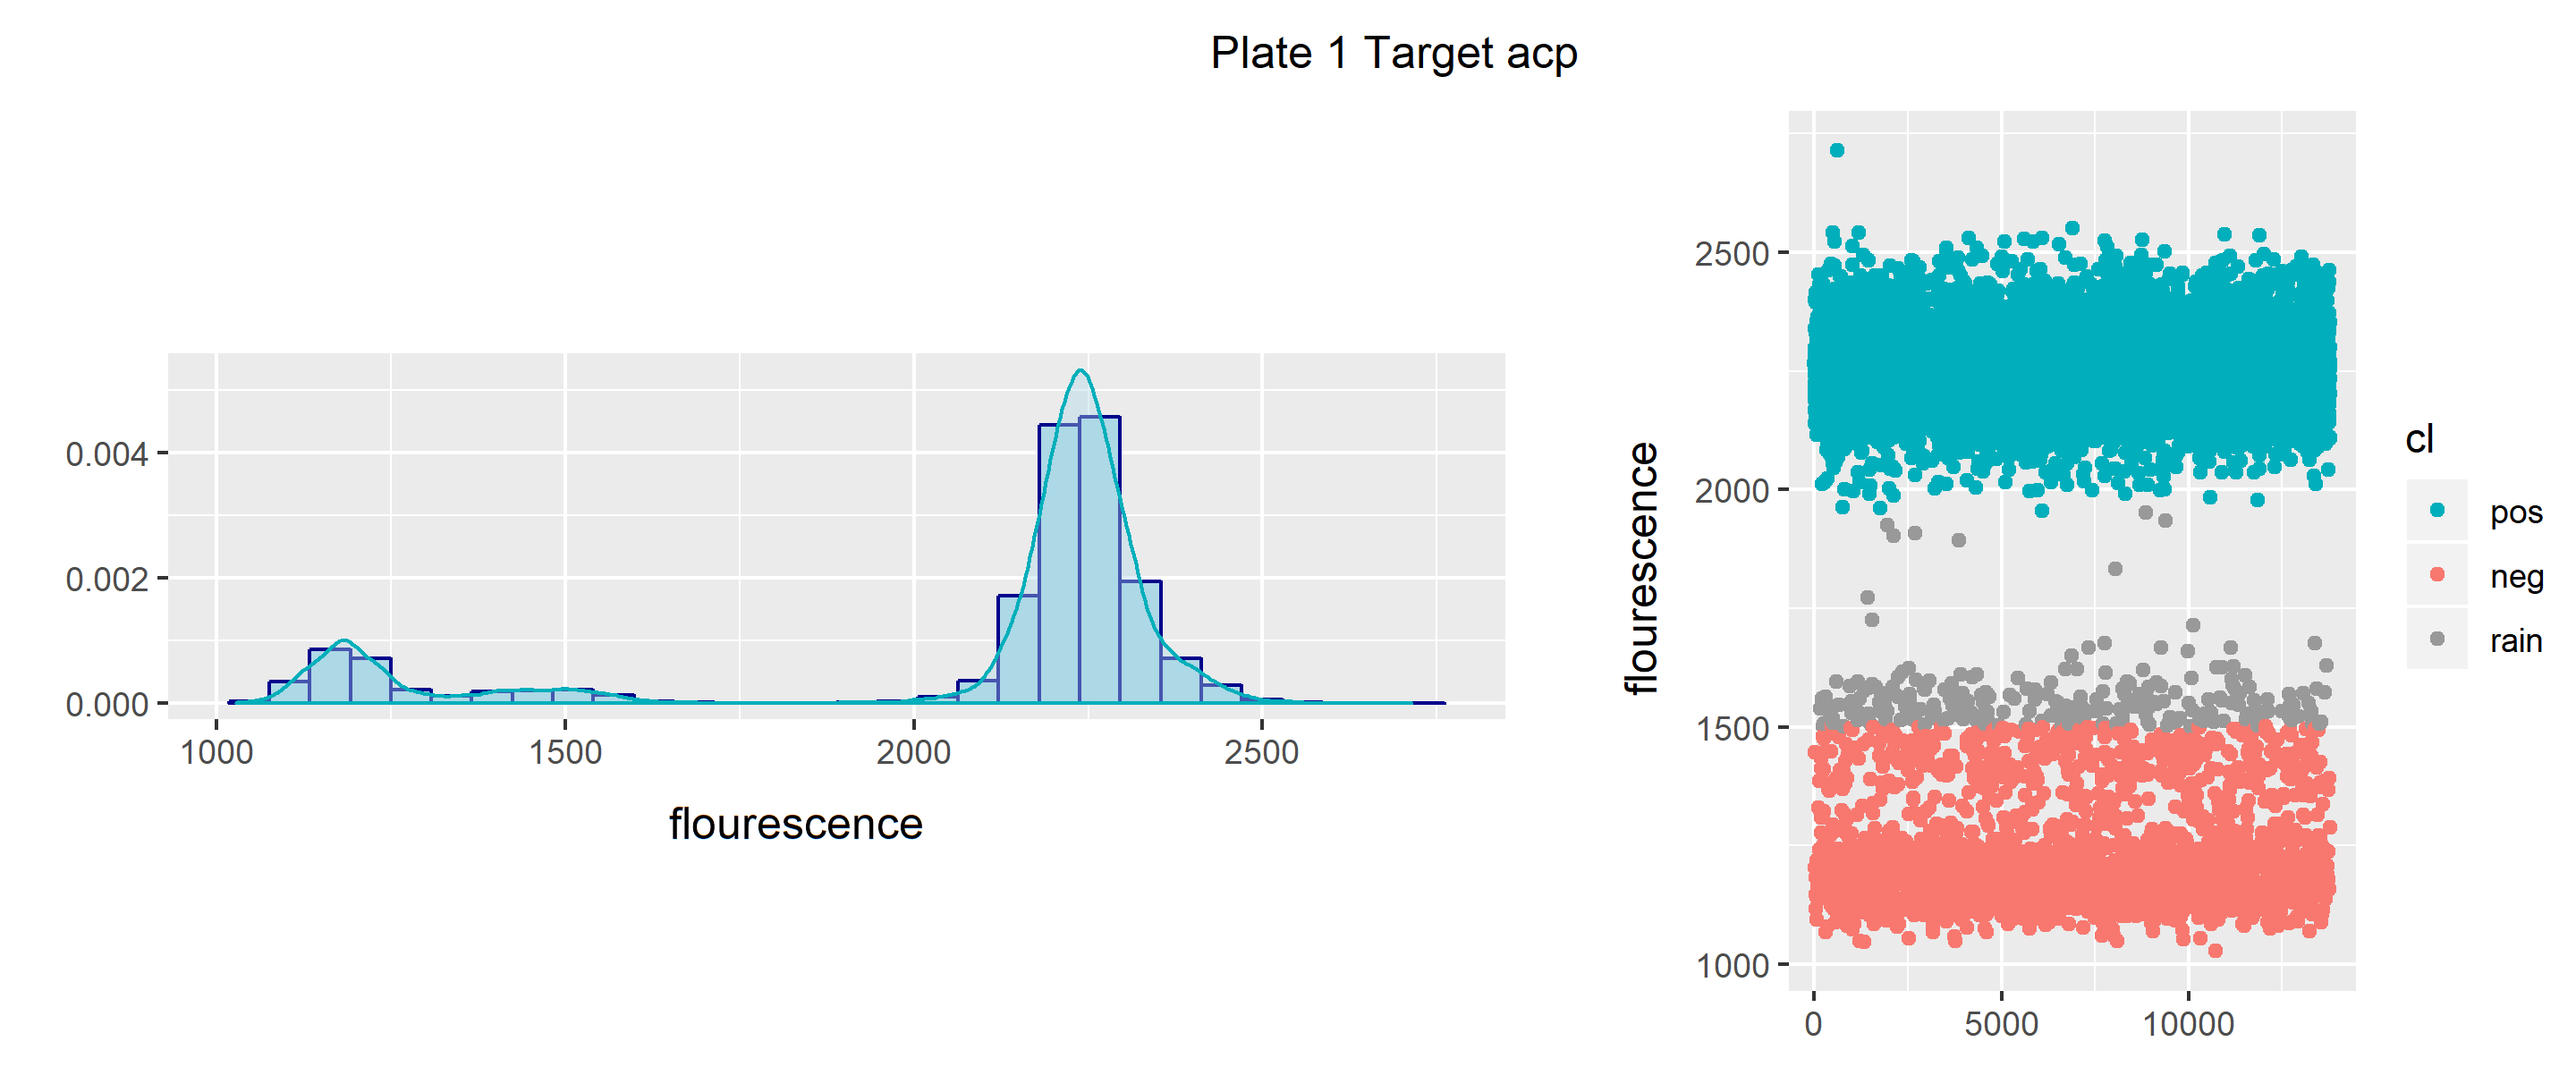
\includegraphics[max size={\textwidth}{\textheight}]{skeweddist.png}
    \caption[Fluorescence distribution of DNA target acp]{One replicate of the DNA target acp Plate 1 from \citeA{Lievens2016} dataset. Left panel shows the fluorescence densities. Right panel is the result of droplet categorization using cloudy}
        \label{fig:skeweddist}
\end{figure}

It is noted that the context of the threshold setting here is based on in-house data, and may not necessarily conclude as a classifier for external experiments. In their study, the cloudy algorithm was able to produce estimates for differing PCR experimental factors, such as sonication, PCR enhancers, annealing conditions, and number of cycles, to achieve optimization or diminishing rain droplets for dPCR experiments.


\subsection{Umbrella}
\label{sec:nonparamdensityest}

As opposed to the distance-based clustering in Section \ref{sec:knn}, a probabilistic approach is achieved with model-based clustering. According to \citeA{Mcnicholas2016}, a finite mixture model is a sum of weighted density components. This mixture model has to be appropriate such that its parameters are flexible for fitting the characteristics of the data. In this approach, each unimodal density component are defined as a cluster; and each observation has a calculated probability of it belonging to a cluster. 

The use of mixture models for clustering has been found to have many applications. In an electricity usage profiling study, \citeA{Li2018_gmm} noticed several elongated ellipses in the scatterplot of electricity usage data, urging the use of Gaussian components for their mixture model. In another example, \cite{Choy2017} performed image segmentation using the generalized Gaussian density model, where each cluster formed is interpreted as an object. Their algorithm was able to segment objects such as a starfish, cat, or tree in photographs. Additionally, using genetic data, \citeA{Li2018_mRna} discovered a potential differentially-variable microRNA (miRNA) not yet reported in literature, upon fitting a three-component multivariate normal distribution to miRNA expression levels. The assumption of the Gaussian component distributions are common in model-based clustering; however, in the succeeding texts, dPCR droplet fluorescence populations are claimed to be not normally distributed. 

In the application dPCR, \shortciteA{Jacobs2017} developed Umbrella, a model-based clustering for dPCR droplets using nonparametric density estimation (https://github.com/statOmics/umbrella). Umbrella requires a set of representative NTC sample(s), the procedure then follows a series of assumptions and estimations in deriving the final estimated concentration. An oversimplification of the Umbrella procedure are as follows:
\begin{enumerate}
    \item The NTC distribution \(f_0(x)\) is assumed to follow a unimodal distribution. The location and variation is estimated by the mode and mean of absolute deviation (MAD), respectively.
    \item The fluorescence intensitities \(x\) observed in partitions of a target partition set \(A\) is assumed to have a mixture density 
    \[f_A(x) = p_{0,A}f_{0,A}(x) + (1-p_{0,A})f_{1,A}(x)\]
    \begin{itemize}
        \item \(p_{0,A}\) = proportion of negative partitions
        \item \(f_{0,A}(x)\) = densities of the partitions without target copy (null component of the target partition set \(A\))
        \item \((1-p_{0,A})\) = proportion of positive partitions
        \item \(f_{1,A}(x)\) = densities of the partitions with target copy
    \end{itemize}
    \item Begin estimating the parameters by first aligning the modes of  the null component of \(f_A(x)\) and the NTC reference \(f_0(x)\).
    \item Discretize the aligned distributions by generating a histogram with the same bins.
    \item The bin counts of the aligned distribution are modeled using a Poisson regression model, resulting in estimates for \(\hat{p}_{0,A}\),\(\hat{f_{0}}(x)\), and \(\hat{f_{A}}(x)\).
    \item The posterior probability that partition \(i\) is void of the NA target with fluorescence intensity \(x_i\) of partition set \(A\), \(\hat{p_{0,A}}\), can be defined from the estimated \(\hat{p}_{0,A}\) from the previous step as
    \[ \hat{p}_{i,0,A}=\hat{p}_{0,A}\left(\begin{array}{c}\hat{f}_{0,A}(x_i)\\ \hat{f}_{A}(x_i)\end{array}\right) \]
    \item The Umbrella threshold estimator is then determined by the estimated \(\hat{p}_{i,0,A}\). For intensity value \(i\), the interpretation of the posterior probabilities are 
    \begin{itemize}
        \item \(\hat{p}_{i,0,A} > 80\%\) are considered negative partitions with a probability of \(\leq20\%\) to be false negatives
        \item \(\hat{p}_{i,0,A} < 5\%\) are considered positive partitions with a probability of \(\leq5\%\) to be false positives
        \item \(5\% \leq \hat{p}_{i,0,A} \leq 80\%\) are considered as rain
    \end{itemize}
\end{enumerate}

The mode and MAD, which estimates the location and spread for the null NTC distribution, \(f_{0}(x)\), are chosen due to its robustness and insensitivity to skewed tails. Only observations within 10 deviations of the mode are included for the null model.

Following the assumption of a mixture density in step 2, unlike most model-based clustering algorithms, Umbrella does not assume normal densities for \(f_{1,A}(x)\) and \(f_{0,A}(x)\), the partitions with and without the nucleic acid target, respectively. This is due to the exhibition of dPCR fluorescence intensities to be non-normal, as clusters tend to have heavy tails to the left or to the right. The solution for this is the use of non-parametric density estimation in step 3.

After estimating all the components in the mixture model from steps 3 - 5, the component of interest \(\hat{p_{0,A}}\) is then used to determine \(\hat{p}_{i,0,A}\) in step 6. Finally, this is used as the basis for Umbrella threshold estimator in step 7. It is warned that Umbrella may not be precise in detection experiments for low copy samples, as classifying individual samples is not the strength of this method.

\subsection{ddpcRquant}
\label{sec:ddpcrquant}
The ddpcRquant determines a threshold for negative droplet fluorescence based on extreme value theory. It is available as an R library developed by Trypsteen et. al (2015). The extreme value theory assumes that the maxima distribution of large samples are distributed as a generalized extreme value (GEV), regardless of the original value's distribution. Hence, the extreme value theory is considered as asymptotically nonparametric provided that samples are sufficiently large. Applying this theory in dPCR droplet classification, an extreme value percentile of the merged NTC samples are used to calculate the threshold. The summarized steps of ddpcRquant are described below :
\begin{enumerate}
    \item The required NTC sample inputs are baseline corrected. This is done subtracting the fluorescence intensities of each sample by the Robertson-Cryer estimated mode.
    \item The fluorescence of all NTC samples are merged, and then randomly assigned to equally sized \(k\) groups, 
    \item Using the maxima of all \(k\) groups, the generalized extreme value distribution is fitted by maximum likelihood.
    \item The tentative threshold is then the 0.995 percentile of this distribution.
    \item The final threshold is the average of all thresholds upon 100 repeats of steps 2-4.
    \item To correct for the baseline of target samples, each sample is subtracted by its fluorescence mode below a cutoff \(c\) — calculated as the average of the NTC modes plus the final threshold.
    \item Finally, to calculated the target concentration, negative and positive droplets are separated using the final threshold from the baseline-corrected target samples. 
\end{enumerate}

The advantages of ddpcRquant are that it doesn't assume any distribution of the droplet fluorescence, corrects for baseline shifts.  In calculating the target concentration, it does not discard any droplet as it states can underestimate the true concentration.

According to the authors' evaluation, ddpcRquant is superior to QuantaSoft in regards to having less false positive counts in the NTC samples, as a consequence, QuantaSoft concentration estimates are generally higher as it identifies more positive droplets. The reason was found to be that Quantasoft places its threshold too close to the negative droplet population, and may be caused by no baseline correction between NTC and target samples, and by its assumption of NTC being normally distributed without fitting experiments. Additionally, QuantaSoft fails to quantify concentration in some samples that result in "No call" outputs.


\section{Expectation-Maximization (EM) Clustering}
\label{sec:emclustering}

Recall from Section \ref{sec:nonparamdensityest}, model-based clustering refers to fitting a finite mixture model given the data set \(X\); then the cluster membership of observation \(x_i\) is determined by the highest probability of it belonging to a density component. Building the mixture model \(f(x|\Theta)\) requires the determination of 1) \(G\) — the number of mixture components (clusters) and 2) \(f_g(x|\theta_g)\) — the distribution assumed to be followed by the mixture component \(g\). 

A common method for determining \(G\) is by selecting the model with the lowest Bayesian Information Criterion (BIC) amongst the proposed \(G\)-component mixture models. As mentioned in the model-based clustering examples in Section \ref{sec:nonparamdensityest}, the mixture components are frequently assumed to follow a Gaussian distribution, and is also known as Gaussian Mixture Model (GMM). Although popular, GMMs poorly fit the data that exhibit skewness and different levels of kurtosis, consequently leading to overestimation on the number of clusters \cite{Dang2019}. Alternatively, the following distributions can better generalize these kinds of data: multivariate \(t\), skewed-\(t\), multivariate power exponential, variance-gamma, generalized hyperbolic, etc. Unlike Gaussian, these component models are flexible for data with varying tail weight, peakedness, and skewness.

After determining the distribution of \(G\) mixture components, the next problem is on how to estimate its corresponding parameter set \(\Theta*\). Expectation-Maximization (EM), a well-known parameter estimation algorithm, is an iterative procedure that maximizes the likelihood of the parameters given the observed data \cite{Garriga2016}. In the EM procedure, the parameter set is initially guessed and is re-estimated in every iteration of the E-step and M-step, until the parameter set reaches convergence. E-step computes the likelihood weight, or the posterior probability, of each data point \(x_i\) belonging to a component \(g\). M-step re-estimates new parameters that maximize the likelihood of these weights for each component. The result of EM guarantees to reach a local maximum for parametric distributions. The direct application of using the final EM posterior probabilities in assigning data points to groups is called EM Clustering (EMC) \cite{Garriga2016}. 

For dPCR droplets classification, since the groups of interest are the positive and negative droplets, a two-component mixture model suffices. However, observations of dPCR data reveal that three or more populations may form; in this case, \(G\) will have to be determined. Additionally, there is room for research in identifying the fluorescence intensity distribution that will fit the characteristics of the positive/negative groups. Since heavy tails are observed in fluorescence densities in \figref{fig:skeweddist}, distributions have to be explored that may best fit the data. 


\section{Performance Evaluation}
\label{sec:ch2_perfeval_estimates}

\subsection{Essential Metrics for dPCR}
\label{sec:ch2_perfeval_essentialMetrics}
As an emerging technology, the number of researchers adopting to dPCR are increasingly growing, and thus, there is a need to standardize the experimental protocols, information, and metrics that should be included in published works. This necessity lead to the proposed Minimum Information for the Publication of Digital PCR Experiments (dMIQE) Guidelines by \shortciteA{Huggett2013_MIQEGuidelines}. Compliance of the dMIQE guidelines allows dPCR analyses to have data comparability and reproducibility between experiments. The main categories of the dMIQE checklist that requires detailed documentation are the following: (1) experimental design, (2) sample, (3) nucleic acid extraction, (4) dPCR target information, (5) dPCR oligonucleotides, (6) dPCR protocol, (7) dPCR validation, (8) and data analysis. Since this paper focuses on the analysis of endpoint fluorescence data, only the metrics in data analysis is further explored.

The data analysis section lists the dPCR metrics that are either essential or desired. Some of the essential metrics are as follows: (1) mean copies per partition, denoted as \(\lambda\), (2) results of positive and negative control samples, (3) repeatability (intraassay variation), (4) and experimental variance or confidence intervals (CI); on the other hand, the desirable metrics include (1) reproducibility (interassay/user/lab etc. variation), and (2) number and concordance of biological replicates. 

An important metric is the \(\lambda\), which denotes the mean number of copies per partition. Reporting \(\lambda\) is emphasized since this is an important factor that determines the precision of the estimate. To calculate \(\lambda\) with accuracy, the three assumptions must be followed \cite{Kreutz2011}:
\begin{enumerate}
    \item Target molecules are homogeneous in a sample and are distributed randomly in partitions of equal volume,
    \item At least one target molecule in a partition is necessary and sufficient for a positive signal,
    \item Target molecules are independent in a sense that there is no interaction with one another or on device surfaces.
\end{enumerate}

When these assumptions are satisfied, the Poisson distribution can be used to derive the formula \(\lambda = -ln(1-k/n)\); where \(k\) is the number of successes in \(n\) trials. In this context, a positive droplet is considered as a success and the total number of droplets or partitions is the number of trails.

% TODO - Include here the derivation of the commonly reported measurement (copies/uL of the stock) %

\subsection{Precision of Quantification Estimates}
\label{sec:ch2_perfeval_essentialMetrics}
As discussed in section \ref{sec:backgroundstudy}, there are numerous sources of variation in the dPCR workflow, including biological, chemical, and operator errors. It is therefore necessary to produce experimental replicates to measure its repeatability (intraassay variation), reproducibility (interassay variation), and experimental variation. Intraassay samples are technical repeats of the same sample and are prepared in the same time and plate. Reproducibility includes the variation from interassay variability (variation added upon repeating an experiment, which includes variation from differing days, times, and plates the assay was prepared), variation from differing operator or laboratory. Experimental variation can be measured when biological replicates are available; if not, an error variance may be estimated using the confidence of interval from the Poisson estimate \cite{Huggett2013_MIQEGuidelines}.

To measure the precision between replicate measurements, the standard deviation, variance, and coefficient of variation (CV) are commonly reported in studies. In a polymavirus study \cite{Arvia2017}, repeatability and reproducibility of a ten-fold serially diluted dPCR assay were measured using the CV of each run's triplicate. Even before dPCR analyses, real-time qPCR has already used CV to measure reproducibility of target concentration estimates and threshold cycles \cite{Cook2009, Lai2003}. The CV is also used to compare the precision of dPCR against real-time qPCR for concentration estimates in several studies. In virology, \shortciteA{Strain2013} observed a lower average CV for dPCR than qPCR for quantifying HIV DNA. A similar finding was shown on cytomegalovirus, \shortciteauthor{Sedlak2014} has reported increased dPCR precision over qPCR through the CVs of the estimated target copies/ml. In the comparative study of \shortciteA{Hindson2013}, they found that in serum miRNAs, dPCR consistently had the lowest average CVs within- and between-runs than qPCR. CVs were used to compare precision across preparative replicates, across RT replicates, and across PCR replicates.

\subsection{Evaluating Unknown Target Concentrations}
\label{sec:ch2_perfeval_essentialMetrics}
Although dPCR is found to be precise, it becomes poor for samples with low molecules per partition and also for samples with high target molecules per positive partition \cite{Huggett2013_MIQEGuidelines}. Because of this limited dynamic range of the instrument, dPCR samples are first diluted. The first use of dilution series to quantitate molecules with Poisson statistics were published by \shortciteA{Sykes1992}. Serial dilution is the stepwise dilution of a substance usually in a geometric progression. In the study of \shortciteauthor{Sykes1992}, a series of 10-fold dilutions of the sample were prepared ranging from \(10^{-4}\) to \(10^{-9}\). Their initial purpose of performing dilution series was to find the optimal point at which the amplification would be distinguishable as positive or negative; recently, researchers have also found the use of dilution factors to estimate the initial target concentration of a sample prior dilution \cite{Gou2018, Zhu2017}. 

The starting target concentration in the sample, denoted as \(c_0\), can be estimated by finding the relationship between \(\lambda\) and \(D\) (serial dilution factor). The mean target copies per partition can also be expressed as \(\lambda = (c_0 \times D)/N \). By taking the logarithms on both sides, \(-\log{-ln(\lambda}) = -\log{D} - \log{\frac{C_0}{N}}\) is derived, and a linear relationship between  \(-\log{-ln(\lambda)}\) and \(-\log{D}\) is established. When a linear regression is fitted, \(C_0\) can be derived using the intercept. In order to compare their dPCR device amongst a commercial dPCR system, \shortciteA{Zhu2017} has used \(C_0\), observing that their device matches the \(C_0\) of the commercial system. In addition, they have also recorded the CV of the replicates for each dilution step. Besides estimating \(C_0\), \shortciteA{Gou2018} has also utilized this linear model to assess the validity of their proposed dPCR devices, wherein a strong linear relationship between \(-\log{-ln(\lambda)}\) and \(-\log{D}\) implies good detection within a dynamic range. \shortciteauthor{Gou2018} have claimed that their device is a robust tool for detection and quantification upon finding an \(R^2\) of 0.9994 from a four step 10-fold dilution series (\(10\) - \(10^{-4})\) of cDNA samples.

% TODO : Add Persson as another example on regressing concentration by dilution factor %

\subsection{Evaluating Known Target Concentrations}
\label{sec:ch2_perfeval_essentialMetrics}
In specific situations, the starting target concentration in a sample is known as prepared by a researcher, these samples are known as a positive control sample. In their evaluation of 'definetherain', a dPCR quantification system with focus on low-copy counts \cite{Jones2014}, a positive control sample was prepared for two targets, albumin and HIV-1 proviral DNA, with expected concentrations of \(10^5\) to \(10^0\) copies. The estimates of 'definetherain' and QuantaSoft were plotted against the expected by regressing \(\log_{10}{(\textup{Expected} + 1)}\) by \(\log_{10}{(\textup{CopyNumber} + 1)}\). The ideal outcome is a 1:1 correspondence between the expected and resulting estimates. In their first linear regression model, only samples with low expected values were included ($<$3000 copies), this resulted in a much more significant p-value ($<$0.01) for 'definetherain' as compared to QuantaSoft; but when including the whole range of concentrations, the linear relationship becomes insignificant for both methods. This conclusion has supported the advantage of 'definetherain' in low-copy samples through the use of the regression of known concentrations by the estimated target copy counts.

% TODO : Add Jacob's simulated dataset evaluation here % 